\documentclass[10pt,journal]{IEEEtran}

\usepackage[scale=0.8]{geometry}
\usepackage{graphicx}

% This centers the captions
\makeatletter
\long\def\@makecaption#1#2{\ifx\@captype\@IEEEtablestring
\footnotesize\begin{center}{\normalfont\footnotesize #1}
{\normalfont\footnotesize\scshape #2}\end{center}
\@IEEEtablecaptionsepspace
\else
\@IEEEfigurecaptionsepspace
\setbox\@tempboxa\hbox{\normalfont\footnotesize {#1.}~~ #2}
\ifdim \wd\@tempboxa >\hsize
\setbox\@tempboxa\hbox{\normalfont\footnotesize {#1.}~~ }
\parbox[t]{\hsize}{\normalfont\footnotesize \noindent\unhbox\@tempboxa#2}
\else
\hbox to\hsize{\normalfont\footnotesize\hfil\box\@tempboxa\hfil}\fi\fi}
\makeatother

\title{Design and implementation of the $sin$ function for an 8-bit MIPS processor}
\author{Dominik Laskowski, Payom Meshgin, Daniel Ranga, Ming Yang}

\begin{document}
\maketitle

\section{Introduction}

\section{Lookup Table Implementation}

\begin{figure}[h]
\centering
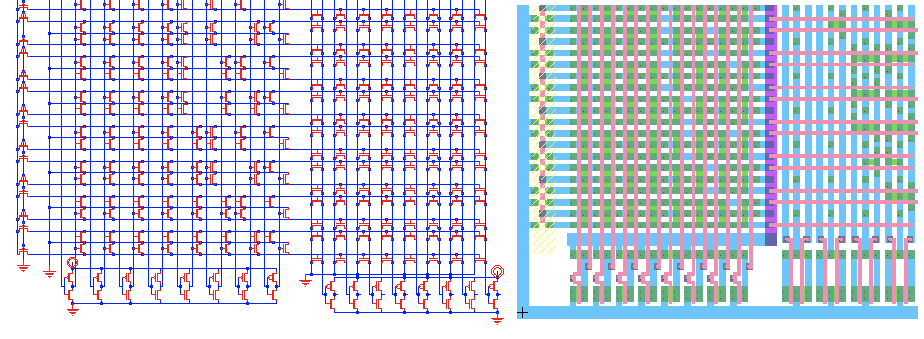
\includegraphics[width=3in]{lut.png}
\caption{Schematic and layout of the lookup table}
\label{lut}
\end{figure}

\section{Taylor Series Implementation}

\section{MIPS Integration}

\section{Validation}

\section{Results}

\section{Conclusion}

\end{document}
